\documentclass[11pt]{article}
\usepackage[paperwidth=12cm, paperheight=18cm, margin=1cm]{geometry}
\usepackage{amsmath, tikz}
\pagestyle{empty}

\begin{document}
\begin{center}
  {\LARGE\bfseries Benford's Law}\\[4pt]
  {\large Why 1 is the most common first digit}
\end{center}

In populations, river lengths, stock prices and tax returns,
about 30\% of numbers start with 1 and fewer than 5\% with 9.

\section*{The first digit distribution}
\[
  P(d) = \log_{10}\left(1 + \frac{1}{d}\right),
  \qquad d = 1, 2, \dots, 9
\]

\begin{center}
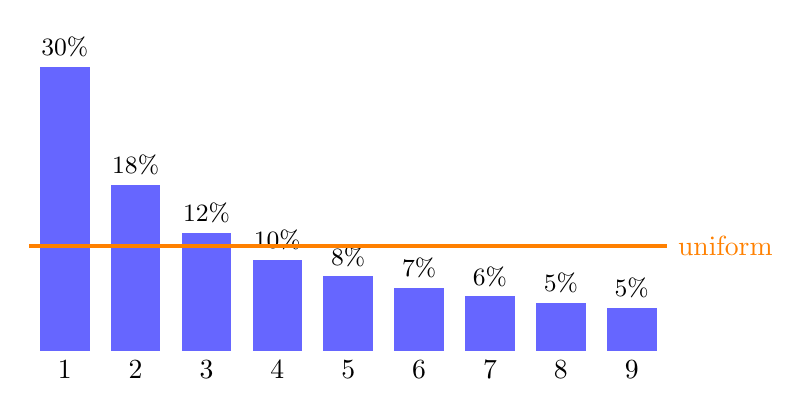
\begin{tikzpicture}[xscale=0.9, yscale=12]
  \foreach \d in {1, ..., 9} {
    \pgfmathsetmacro{\p}{log10(1 + 1/\d)}
    \fill[blue!60] (\d-0.35,0) rectangle (\d+0.35,\p);
    \node[below] at (\d,0) {\d};
    \pgfmathsetmacro{\pct}{round(100*\p)}
    \node[above, font=\small] at (\d,\p) {\pgfmathprintnumber{\pct}\%};
  }
  \draw[orange, very thick] (0.5,1/9) -- (9.5,1/9)
    node[right] {uniform};
\end{tikzpicture}
\end{center}

\section*{Why?}
Numbers that grow by a constant percentage spend the
longest time with leading digit 1: going from 1000 to 2000
means doubling, while 9000 to 10\,000 takes just 11\%.
\[
  \log_{10} 2 - \log_{10} 1 = 0.301
\]
\centerline{\bfseries Auditors use it to catch faked numbers.}
\end{document}
